\documentclass[titlepage,12pt,a4paper,times,oneside]{book}

\usepackage[utf8]{inputenc}
\usepackage[portuguese]{babel}
% substituir linha anterior por 
% \usepackage[english]{babel} 
% se o relatório for escrito na língua inglesa.
\usepackage[T1]{fontenc}
\usepackage{makeidx}
\usepackage{xspace}
\usepackage{graphicx,color,times}
\usepackage{fancyhdr}
% \usepackage{pxfonts}
% \usepackage{times}
% \usepackage{mathptm}
% \usepackage{amssymb}
% \usepackage{amsfonts}
\usepackage{amsmath}
\usepackage{latexsym}
\usepackage[printonlyused]{acronym}
\usepackage{float}
\usepackage{listings}
\usepackage{tocbibind}
\usepackage{wrapfig}
% \usepackage{natbib}
\usepackage{hyperref}
% \usepackage{glossaries}
% \makeglossaries

\usepackage{minted}
\usepackage{paralist}
\usepackage{enumitem}
\usepackage{booktabs}
\usepackage{amssymb}
\usepackage{calc}
\usepackage{array}
\usepackage{color}
\usepackage{colortbl}
% \usepackage{biblatex}

% \renewcommand{\ttdefault}{phv}

\pagestyle{fancy}
\renewcommand{\chaptermark}[1]{\markboth{#1}{}}
\renewcommand{\sectionmark}[1]{\markright{\thesection\ #1}}
\fancyhf{} \fancyhead[LE,RO]{\bfseries\thepage}
\fancyhead[LO]{\bfseries\rightmark}
\fancyhead[RE]{\bfseries\leftmark}
\renewcommand{\headrulewidth}{0.5pt}
\renewcommand{\footrulewidth}{0pt}
\addtolength{\headheight}{0.5pt}
\setlength{\marginparsep}{0cm}
\setlength{\marginparwidth}{0cm}
\setlength{\marginparpush}{0cm}
\addtolength{\hoffset}{-1.0cm}
\addtolength{\oddsidemargin}{\evensidemargin}
\addtolength{\oddsidemargin}{0.5cm}
\addtolength{\evensidemargin}{-0.5cm}


% NEW COLORS
\definecolor{dark}{gray}{0.25}
\definecolor{lgray}{gray}{0.9}
\definecolor{dkblue}{rgb}{0,0.13,0.4}
\definecolor{dkgreen}{rgb}{0,0.6,0}
\definecolor{gray}{rgb}{0.5,0.5,0.5}
\definecolor{mauve}{rgb}{0.58,0,0.82}

\lstset{ %
  language=C,                    basicstyle=\footnotesize,
  numbers=none,                  numberstyle=\tiny\color{gray}, 
  stepnumber=1,                  numbersep=5pt,
  backgroundcolor=\color{white}, showspaces=false,
  showstringspaces=false,        showtabs=false,
  frame=single,                  rulecolor=\color{black},
  tabsize=2,                     captionpos=b,
  breaklines=true,               breakatwhitespace=false,
  title=\lstname,                keywordstyle=\color{blue},
  commentstyle=\color{dkgreen},  stringstyle=\color{mauve},
  escapeinside={\%*}{*)},        morekeywords={*},
  belowskip=0cm
}

\renewcommand{\listingscaption}{Excerto de Código}
\renewcommand{\listoflistingscaption}{Lista de Excertos de Código}% 

\graphicspath{{./img/}}
\newcommand{\usecasescale}{0.5}

\newcommand{\theteam}{Lunáticos}
\newcommand{\theapp}{\emph{Bohr}}
\newcommand{\theappdescription}{Very Small PDB Molecular Visualizer}
\newcommand{\groupname}{{\itshape\theteam}}
\newcommand{\appname}{\emph{\theapp}:~{\emph{\theappdescription}}}
\newcommand{\opengl}{\textit{OpenGL}\textsuperscript{\textregistered}}

\newcommand{\famousquote}[2]{
	\begin{quote}
		\rule{\textwidth-2\leftmargin}{0.4pt}
		{\itshape #1}
		\vspace{-12pt}
		\begin{flushright}
			\textasciitilde~#2
		\end{flushright}
		\vspace{-20pt}
		\rule{\textwidth-2\leftmargin}{0.4pt}
	\end{quote}
}

% \setlist{nosep}


\begin{document}

\thispagestyle{empty}
\setcounter{page}{-1}

\begin{center}
\begin{Huge}
\textbf{Universidade da Beira Interior}
\end{Huge}
\end{center}

\begin{center}
\begin{Huge}
Departamento de Informática
\end{Huge}
\end{center}

\vspace{0,07cm}
\begin{figure}[!htb]
\centering

\includegraphics[width=191pt]{ubi-fe-di.png}
\end{figure}

\vspace{0.5cm}
\begin{center}
\begin{Large}
\textbf{\appname}
\end{Large}
\end{center}

\vspace{0.5cm}
\begin{center}
\begin{normalsize}
\begin{large}
Elaborado por:
\end{large}
\end{normalsize}
\end{center}

\vspace{0.2cm}
\begin{center}
\begin{large}
\begin{tabular}{>{\bfseries}r @{~~---~~} >{\bfseries}l}
	41266 & Diogo Castanheira Simões    \\
	41381 & Igor Cordeiro Bordalo Nunes
\end{tabular}
\end{large}
\end{center}

\vspace{0,5cm}
\begin{center}
\begin{normalsize}
\begin{large}
Orientador:
\end{large}
\end{normalsize}
\end{center}

\vspace{0.2cm}
\begin{center}
\begin{large}
\textbf{Professor Doutor Abel João Padrão Gomes}
\end{large}
\end{center}

\vspace{0.5cm}
\begin{center}
\begin{normalsize}
%\today
14 de Janeiro de 2020
\end{normalsize}
\end{center}

\clearpage{\thispagestyle{empty}\cleardoublepage}

\frontmatter

% \chapter*{Resumo}
\label{ch::resumo}

% 2 frases onde introduzem o tema
Text\ldots

% 2 frases (máximo) onde dizem como abordaram o tema
Text\ldots

% 1 ou 2 frases onde se referem os objetivos ou resultados alcançados
Text\ldots


%\clearpage{\thispagestyle{empty}\cleardoublepage}


\tableofcontents

%\clearpage{\thispagestyle{empty}\cleardoublepage}

\listoffigures

% Se não existirem tabelas, comentar as seguintes linhas
%\clearpage{\thispagestyle{empty}\cleardoublepage}
\listoftables

% Se existirem trechos de código, descomentar as seguintes linhas
% \clearpage{\thispagestyle{empty}\cleardoublepage}
%\listoflistings
%\addcontentsline{toc}{chapter}{\listoflistingscaption}

%\clearpage{\thispagestyle{empty}\cleardoublepage}
\chapter*{Acrónimos}
\label{ch::acro}

\begin{acronym}[ARGB]
	\acro{API}{\textit{Application Programming Interface}}
	\acro{ARGB}{\textit{Alpha-Red-Green-Blue}}
    \acro{CG}{Computação Gráfica}
    \acro{GLM}{\textit{OpenGL Mathematics}}
    \acro{GLSL}{\textit{OpenGL Shader Language}}
    \acro{PDB}{\textit{Protein Database}}
	\acro{SWOT}{\textit{Strength, Weakness, Opportunity, and Threat Analysis}}
	\acro{UC}{Unidade Curricular}
	\acro{URI}{\textit{Uniform Resource Identifier}}
\end{acronym}

% \clearpage{\pagestyle{empty}\cleardoublepage}
% \chapter*{Glossário}
\makeglossaries

\newglossaryentry{.NET Framework}
{
  name={.NET Framework},
  description={É uma plataforma para desenvolvimento e funcionamento de aplicações desenvolvida pela Microsoft.}
}

\newglossaryentry{ASP.NET}
{
  name={ASP .Net},
  description={É uma plataforma da Microsoft para o desenvolvimento de aplicações Web e é o sucessor da tecnologia ASP.}
}

\newglossaryentry{CS}
{
  name={C\#},
  description={Lê-se \textit{C Sharp} e é uma linguagem de programação orientada a objectos, desenvolvida pela Microsoft, inicialmente para a plataforma .NET. O C\# é inspirado na junção entre as linguagens C++ e Java.}
}


\newglossaryentry{Java}
{
  name={JAVA},
  description={É uma linguagem de programação orientada a objectos, desenvolvida pela Sun Microsystems na década de 90. Hoje pertence à empresa Oracle.}
}


\newglossaryentry{OpenDMTP}
{
  name={OpenDMTP},
  description={\textit{Open Device Monitoring and Tracking Protocol} é um protocolo e uma \textit{framework} abertos que permite a comunicação bidireccional entre servidores e clientes através da internet.}
}


\newglossaryentry{OpenGTS}
{
  name={Open GTS},
  description={É o primeiro projecto \textit{Open Source} \textit{Web-Based} para controlo de frotas por GPS.}
}


\newglossaryentry{VS2010}
{
  name={Visual Studio 2010},
  description={\textit{Microsoft Visual Studio 2010} é um sistema de desenvolvimento desenvolvido pela Microsoft e é dedicado ao Framework .NET, que contem um conjunto de ferramentas de desenvolvimento projectadas para auxiliar os programadores a enfrentarem desafios complexos.}
}


\newglossaryentry{WebS}
{
	name={Web Service},
	description={Web services são aplicações modulares auto-descritas e auto-contidas, que permitem a integração de sistemas e a comunicação entre aplicações de diferentes tipos.}
}


\newglossaryentry{WebBased}
{
	name={Web Based},
	description={Aplicação desenvolvida para a Web.}
}

\newglossaryentry{Roaming}
{
	name={Roaming},
	description={Define a possibilidade de um utilizador de uma determinada rede obter rede/conecção fora da área geográfica onde foi registado.}
}


\newglossaryentry{Smartphone}
{
	name={Smartphone},
	description={Smartphone é um telefone móvel que contem muitas das principais tecnologias de comunicação e serviços que existem nos computadores pessoais, como acesso a e-mails, serviços de mensagens instantâneas, internet, GPS, entre outros.}
}

\newglossaryentry{TCPIP}
{
	name={TCP/IP},
	description={É um conjunto de protocolos de comunicação entre computadores ligados rede. O nome TCP/IP surge da união entre dois protocolos: o TCP (Transmission Control Protocol) e o protocolo IP (Internet Protocol).}
}

\newglossaryentry{Firewall}
{
	name={Firewall},
	description={É o nome criado para definir um dispositivo para uma rede de computadores que tem como objectivo criar uma política de segurança num determinado ponto de controlo da rede.}
}

\newglossaryentry{JavaScript}
{
	name={JavaScript},
	description={É uma linguagem de programação baseada na linguagem de programação ECMAScript. Actualmente é a linguagem de programação mais utilizada em \textit{``Client-Side''} nos \textit{browsers}.}
}

\newglossaryentry{Flash}
{
	name={Flash},
	description={Desenvolvido pela Macromedia, o Flash é um software utilizado para criação de animações interactivas que funcionam incorporadas em \textit{Browsers}, \textit{Desktop}, \textit{Smartphones}, \textit{Tablets}, e Televisores.}
}


\newglossaryentry{StoredProcedure}
{
	name={Stored Procedure },
	description={É o nome dado a um conjunto de comandos numa base de dados de forma a simplificar a sua utilização.}
}

\newglossaryentry{SQLS}
{
	name={SQL Server 2008},
	description={É um sistema de gestão de base de dados relacional criado pela Microsoft.}
}

\newglossaryentry{Firm}
{
	name={Firmware},
	description={É o conjunto de instruções operacionais programadas directamente no \textit{hardware} de um equipamento electrónico.}
}

\newglossaryentry{browser}
{
	name={Browser},
	description={É um programa de computador que possibilita aos utilizadores uma interacção com documentos virtuais da Internet, também conhecidos como páginas Web.}
}



%\clearpage{\thispagestyle{empty}\cleardoublepage}

\mainmatter
\acresetall
\chapter{Introdução}
\label{chap:intro}

\section{Descrição da proposta}
\label{sec::intro:descricao}

Várias áreas científicas de elevada importância na sociedade moderna dependem do estudo ao nível molecular e atómico dos componentes que sustentam a vida na Terra. Entre elas destacam-se em particular a indústria farmacêutica, a biotecnologia e as áreas afetas como a química orgânica.

Contudo, apesar da existência de vários \textit{softwares} no mercado para a visualização e estudo destas, é de grande interesse na área da \ac{CG} perceber como se pode renderizar estas moléculas de forma a poderem ser observadas virtualmente e estudadas.

Neste sentido, o grupo desafiou-se a desenvolver um visualizador molecular simplificado de ficheiros \ac{PDB} no âmbito da \ac{UC} de \ac{CG} ao invés dos projetos clássicos propostos inicialmente.

A proposta inicial consiste num visualizador molecular que renderize a superfície implícita \textit{pi} \cite{DBLP:journals/corr/abs-1906-06751}. Contudo, devido a contratempos descritos \textit{a posteriori} no presente documento, a implementação final centra-se na renderização da superfície de \textit{van der Walls}.


\section{Constituição do grupo}
\label{sec::intro:grupo}

O presente projeto foi realizado pela equipa constituída pelos elementos listados na Tabela \ref{tab::team}. O trabalho realizado por cada membro é descrito na Secção \ref{sec::reflexao:divisao}.

\begin{table}[!h]
	\centering
	\begin{tabular}{c l}
		\toprule
		\textbf{N\textordmasculine} & \textbf{Nome} \\
		\midrule
		41266 & Diogo Castanheira Simões    \\
		41381 & Igor Cordeiro Bordalo Nunes \\
		\bottomrule
	\end{tabular}
	\caption[Constituição do grupo]{Constituição do grupo.}
	\label{tab::team}
\end{table}


\section{Organização do Documento}
\label{sec::intro:organizacao}
% !POR EXEMPLO!
De modo a refletir o projeto realizado, este relatório encontra-se estruturado em cinco capítulos:

\begin{enumerate}
\item No primeiro capítulo --- \textbf{Introdução} --- é apresentado o projeto, em particular os seus objetivos, a equipa desenvolvedora, a respetiva organização do relatório e um breve resumo do Estado da Arte do tema por si abordado.

\item No segundo capítulo --- \textbf{Tecnologias utilizadas} --- são delineadas as tecnologias utilizadas durante o seu desenvolvimento.

\item No terceiro capítulo --- \textbf{Desenvolvimento e Implementação} --- são descritas as escolhas e os detalhes de implementação da aplicação.

\item No quarto capítulo --- \textbf{Reflexão Crítica e Problemas Encontrados} --- são indicados os objetivos alcançados, quais as tarefas realizadas por cada membro do grupo, assim como são expostos os problemas enfrentados e é feita uma reflexão crítica sobre o trabalho.

\item No quinto capítulo --- \textbf{Conclusões e Trabalho Futuro} --- são analisados os conhecimentos adquiridos ao longo do desenvolvimento do projeto e, em contrapartida, o que não se conseguiu alcançar e que poderá ser explorado futuramente.
\end{enumerate}


\section{Resumo do Estado da Arte}
\label{sec::intro:estado-arte}

Text\ldots
%\clearpage{\thispagestyle{empty}\cleardoublepage}
\chapter{Tecnologias utilizadas}
\label{ch::tecno}


\section{Introdução}
\label{sec::tecno:intro}

Antes da implementação propriamente dita da aplicação, é necessário estabelecer quais as ferramentas e as tecnologias utilizadas a fim de alcançar os objetivos propostos para o projeto. Este Capítulo aborda, portanto, este tópico.


\section{Ferramentas e tecnologias utilizadas}
\label{sec::tecno:tecnologia}

As ferramentas utilizadas no âmbito da realização do projeto, sumariadas na Tabela \ref{tab::ferramentas}, visam três componentes essenciais na sua gestão:
\begin{inparaenum}[1)]
	\item aplicação \opengl,
	\item relatório, e
	\item controlo de versões.
\end{inparaenum}

Segue-se uma descrição do uso de cada uma das tecnologias:

\begin{itemize}
    \item \textbf{\opengl~\cite{opengl}}: \ac{API} multi-plataforma e com suporte a múltiplas linguagens de programação para a renderização de gráficos vetoriais 2D e 3D com recurso à placa gráfica;
    
    \item \textbf{GLFW~\cite{glfw}}: \ac{API} simplificada para o \opengl, igualmente multi-plataforma, permitindo a gestão de janelas, contextos, superfícies e comandos (rato, teclado e \textit{joystick});
    
    \item \textbf{GLM~\cite{glm}}: biblioteca matemática baseada na linguagem dos \textit{shaders} do \opengl, \ac{GLSL}.
    
    \item \textbf{\ac{GLAD}~\cite{glad,glad-webservice}}: gerador automático de \textit{loaders} para \opengl;
    
    \item \textbf{\textit{FreeType}~\cite{freetype}}: biblioteca de desenvolvimento dedicada à renderização de fontes em \textit{bitmaps} utilizáveis, por exemplo, pelo \opengl.
\end{itemize}

\begin{table}[!htbp]
    \centering
    \begin{tabular}{p{1cm} l l}
        \toprule
        & {\bfseries \textit{Software} / Tecnologia} & {\bfseries Versão} \\
        \midrule
        \multicolumn{3}{l}{\bfseries Aplicação \opengl} \\
        & \opengl           & 4.6 \\
        & GLFW              & 3.3.2 \\
        & GLAD              & 0.1.34 \\
        & \acs{GLM}         & 0.9.9.8 \\
        & \textit{FreeType} & 2.10.4 \\
        \midrule
        \multicolumn{3}{l}{\bfseries Relatório} \\
        & Xe\TeX & 3.14159265-2.6-0.999991 \\
        & \textit{TeXstudio}\textsuperscript{\textcopyright} & 3.0.1 \\
        \midrule
        \multicolumn{3}{l}{\bfseries Controlo de versões} \\
        & \textit{git} & 2.17.1 \\
        & \textit{GitKraken} & 7.4.1  \\
        \bottomrule
    \end{tabular}
    \caption[Ferramentas utilizadas]{Ferramentas e tecnologias utilizadas, organizadas por categoria.}
    \label{tab::ferramentas}
\end{table}


\section{Código \textit{open source}}

Foi utilizado código \textit{open source}, adaptado para o projeto sob as respetivas licenças, para as seguintes funcionalidades:

\begin{itemize}
    \item \textbf{\itshape Sphere}~\cite{glsl-cookbook-github,vbosphere}: obtido dos códigos de exemplo do \textit{OpenGL Shading Language Cookbook, 2nd Edition} para renderizar esferas sem recurso a ficheiros \verb*|*.obj| criados externamente;
    
    \item \textbf{\itshape osdialog}~\cite{osdialog}: biblioteca multi-plataforma para acesso facilitado às caixas de diálogo do sistema operativo, com o fim de permitir abrir qualquer ficheiro \ac{PDB} dinamicamente a qualquer momento e mostrar mensagens de erro ao utilizador.
\end{itemize}

O projeto \theapp~será por sua vez disponibilizado sob a licença \textit{GNU General Public License, version 3}~\cite{gnugpl3}, após apresentação e caso seja autorizado pelo Professor regente.


\section{Conclusões}
\label{sec::tecno:conclusao}

Após delineadas as ferramentas e tecnologias a utilizar, segue-se a fase de desenvolvimento do projeto, descrito no Capítulo seguinte. A utilização de código \textit{open source} e de ferramentas bem conhecidas e testadas pela comunidade mundial permitirá, em princípio, uma implementação eficiente.

%\clearpage{\thispagestyle{empty}\cleardoublepage}
\chapter{Desenvolvimento e Implementação}
\label{ch::implement}

\section{Introdução}
\label{sec::implement:intro}

A fase de implementação, que se estendeu por cerca de 2 semanas, envolveu a execução paralela de diferentes tarefas pelos dois elementos do grupo. Este Capítulo aborda em particular os seguintes aspetos desta fase do projeto:

\begin{itemize}%[nosep]
	\item Escolhas de implementação (Secção \ref{sec::implement:escolhas}): explica as decisões feitas durante a implementação do código-fonte;
	\item Detalhes de implementação (Secção \ref{sec::implement:detalhes}): explora os detalhes mais importantes e/ou interessantes no código-fonte.
\end{itemize}

Adicionalmente, são descritos o manual de instalação (Secção \ref{sec::implement:instalar}) e %: aborda a compilação da aplicação e a respetiva instalação num \textit{smartphone} com sistema operativo \textit{Android}\texttrademark;
o manual de utilização (Secção \ref{sec::implement:utilizacao}). %: exemplifica o uso da aplicação final na ótica do utilizador.


\section{Escolhas de Implementação}
\label{sec::implement:escolhas}

A primeira e grande escolha de implementação que se faz notar ao longo de todo o código é a utilização de classes e das bibliotecas providenciadas pelo C++ a fim de tirar o máximo partido desta linguagem de programação.

Desta forma, o código-fonte está organizado nas seguintes pastas:

\begin{itemize}
    \item \verb|bin|: inclui o binário compilado e as seguintes pastas:
    \begin{itemize}[nosep]
        \item \verb|fonts|: localização das fontes utilizadas para renderizar texto;
        \item \verb|shaders|: alberga os \textit{fragment shaders} e os \textit{vertex shaders} para a renderização das moléculas e do texto.
    \end{itemize}
    \item \verb|deps|: pasta gerada pelo \textit{Makefile} para gerir as dependências durante a compilação;
    \item \verb|doc|: aloja a documentação do projeto (nomeadamente o presente relatório);
    \item \verb|include|: pasta com os \textit{header files} de todos os métodos e classes utilizados no projeto;
    \item \verb|obj|: pasta gerada pelo \textit{Makefile} para guardar os ficheiros objeto a serem compilados no executável final;
    \item \verb|src|: alberga todos os códigos-fonte (ficheiros \verb|*.cpp|) com a implementação dos métodos e das classes declaradas nos \textit{header files} da pasta \verb|include|.
\end{itemize}


\section{Detalhes de Implementação}
\label{sec::implement:detalhes}

O ficheiro principal, \verb|bohr.cpp|, aloja a função \verb|main()| de onde o programa arranca. Aqui são invocadas as seguintes funções de inicialização:

\begin{minted}[breaklines,linenos]{cpp}
GLFWwindow* initialize_glfw(int width, int height, const char* title);
int initialize_glad(void);
\end{minted}

Estas funções inicializam, respetivamente, as bibliotecas GLFW e GLAD, necessárias para a comunicação com a \ac{API} do \opengl. Caso a primeira função retorne \verb|NULL| ou a segunda retorne \verb|0|, é gerada uma mensagem de erro na linha de comandos e o programa é abortado. A função de inicialização do GLFW em particular associa as funções de \textit{callback} para o teclado e para o rato.

De seguida são compilados os \textit{shaders} de renderização das moléculas com recurso à classe \textit{Shader} (implementada em \verb|shader_m.cpp|):

\begin{minted}[breaklines,linenos]{cpp}
debug("Loading shaders...\n");
Shader lightingShader = Shader("shaders/lighting_vs.glsl", "shaders/lighting_fs.glsl");
\end{minted}

Esta classe fornece métodos rápidos e muito acessíveis para manipular os dados passados aos \textit{shaders} e a respetiva utilização.

É ainda inicializado o renderizador de texto:

\begin{minted}[breaklines,linenos]{cpp}
TextRenderer textrenderer = TextRenderer(SCR_WIDTH, SCR_HEIGHT);
try {
    textrenderer.Load("fonts/UbuntuMono-R.ttf", 24);
} catch (const std::exception &e) {
    std::cerr << e.what() << '\n';
}
\end{minted}

A classe \textit{TextRenderer} está disponível \textit{online} \cite{textrender} para livre utilização, assim como os \textit{shaders} para a renderização deste mesmo texto.

Por fim, o programa entra no seu ciclo de renderização. Este começa por limpar o \textit{buffer} atual e renderiza os textos, nomeadamente as instruções no canto superior esquerdo e o nome do ficheiro (se aberto) no canto inferior esquerdo.

De imediato é processado o \textit{input} de teclado do utilizador com a seguinte função:

\begin{minted}[breaklines,linenos]{cpp}
action processInput(GLFWwindow *window, char **fname);
\end{minted}

Esta função ajusta os parâmetros da câmara conforme as teclas selecionadas, mas em particular trata de abrir a janela de diálogo para abrir um ficheiro novo com o seguinte excerto de código:

\begin{minted}[breaklines,linenos]{cpp}
if (glfwGetKey(window, GLFW_KEY_O) == GLFW_PRESS) {
    switchModeView(window, false);
    if (*fname != NULL) free(*fname);
    *fname = openPDBFileDialog();
    switchModeView(window, true);
    return (*fname != NULL) ? action::OPEN_FILE : action::NO_ACTION;
}
\end{minted}

O modo de visualização é temporariamente alterado a fim de permitir que o cursor do rato seja visível durante a seleção do ficheiro uma vez que este é oculto durante a renderização da molécula. Após obter o caminho para o ficheiro pretendido, a função verifica se porventura não será \verb|NULL|: neste caso, a molécula renderizada atualmente mantém-se e não é apagada da memória. Caso contrário, é devolvido um enumerador do tipo \verb|action| que indica que o utilizador selecionou um novo ficheiro:

\begin{minted}[breaklines,linenos]{cpp}
typedef enum {
    NO_ACTION,
    CAMERA_RESET,
    OPEN_FILE
} action;
\end{minted}

No ciclo de renderização é feita uma análise deste retorno a fim de determinar a próxima ação. O \textit{reset} da câmara envolve a invocação da seguinte chamada:

\begin{minted}[breaklines,linenos]{cpp}
camera = molecule.resetCamera();
\end{minted}

Esta função será vista mais à frente.

Caso seja aberto um novo ficheiro, a sua extensão é verificada como forma de validação primária:

\begin{minted}[breaklines,linenos]{cpp}
bool isPBD(char *fname) {
    return
    string(std::experimental::filesystem::
        path(fname).extension())
        .compare(".pdb") == 0;
}
\end{minted}

Sendo um ficheiro \ac{PDB}, a seguinte linha de código irá carregar uma nova molécula a partir do ficheiro selecionado pelo utilizador:

\begin{minted}[breaklines,linenos]{cpp}
    molecule = Molecule().fromPDB(fname);
\end{minted}

Por fim, a molécula é renderizada de forma a apresentar a superfície de \textit{van der Walls}:

\begin{minted}[breaklines,linenos]{cpp}
molecule.render_vanderWalls(lightingShader, camera, screen_width, screen_height, molrotx, molroty);
\end{minted}

À classe \textit{Molecule}, implementada no ficheiro \verb|pdbreader.cpp|, são delegadas todas as seguintes tarefas:

\begin{itemize}
    \item Ler o ficheiro \ac{PDB} e fazer o respetivo \textit{parsing} a fim de obter os átomos e as respetivas coordenadas;
    
    \item Obter os dados relativos a cada átomo dada a tabela periódica implementada em \verb|ptable.h|, nomeadamente o raio de \textit{van der Walls} \cite{ptable} e a cor CPK \cite{cpk};
    
    \item Computar as esferas associadas a cada átomo dado o raio determinado anteriormente;
    
    \item Renderizar as esferas nas posições correspondentes às coordenadas do respetivo átomo e com a respetiva cor;
    
    \item Determinar a posição inicial da câmara dada a dimensão da molécula processada através do método \verb|resetCamera()|.
\end{itemize}

Após estudo do formato de ficheiros \ac{PDB}, determinou-se que o \textit{parsing} seria simplificado uma vez que as posições de cada dado é esperado exatamente sempre na mesma posição de cada linha, em particular:

\begin{itemize}
    \item Três coordenadas nas posições 30, 38 e 46 da linha;
    \item Símbolo atómico na posição 76.
\end{itemize}

Só as linhas começadas por \verb|ATOM| ou \verb|HETATM| são interpretadas uma vez que são estas aquelas que contêm os dados relativos aos átomos. Uma vez que só é pretendida a superfície, não é necessário calcular as ligações entre átomos (o formato \ac{PDB} não fornece esta informação explicitamente).

Dada a política determinada anteriormente na Secção \ref{sec::implement:escolhas}, a classe \textit{Molecule} \textbf{não} é responsável por calcular os pontos das esferas. Uma classe própria existe para o efeito, \textit{VBOSphere}, sendo então criadas instâncias desta classe num vetor:

\begin{minted}[breaklines,linenos]{cpp}
bool Molecule::generateSpheres(void) {
    this->spheres = vector<VBOSphere>();
    for (auto atom : this->atoms) {
        this->spheres.push_back(VBOSphere(atom.radius, 50, 50, PeriodicTable::getColorFromSymbol(atom.name)
            .toVec3()));
    }
    return true;
}
\end{minted}

Classes e estruturas (\textit{structs}) foram criadas para lidar com pontos e cores a fim de fornecer métodos imediatos para os converter no tipo de dados \verb|glm::vec3| através da função \verb|toVec3()|, comum a ambas as classes.

A renderização da molécula passa por um ciclo que percorre todas as esferas anteriormente computadas, carregando no respetivo \textit{shader} a cor de cada esfera e a posição da câmara como fonte de luz. É de igual forma feita a transformação no mundo através de rotação, translação e escala (exatamente por esta ordem) a fim de posicionar a esfera no local exato. Bastará nesta fase invocar o seguinte método:

\begin{minted}[breaklines,linenos]{cpp}
this->spheres[i].render();
\end{minted}

O resultado final é semelhante ao do exemplo da Figura \ref{fig::bohr-main}.


\section{Manual de Instalação}
\label{sec::implement:instalar}

O projeto foi implementado primariamente para o sistema operativo \textit{Linux}. Em especial, foi utilizado o \textbf{\textit{Linux Mint} 20.0} com as mais recentes atualizações em dia.

A fim de compilar o projeto, é necessário ter as seguintes bibliotecas instaladas no sistema:

\begin{itemize}[nosep]
    \item \verb|g++|;
    \item \verb|make|;
    \item \verb|libglfw3-dev|;
    \item \verb|libglm-dev|;
    \item \verb|freetype|.
\end{itemize}

O \textit{Makefile} incluído tratará da compilação de todos os ficheiros de forma automática, sendo fornecidos três modos:

\begin{enumerate}
    \item \verb|make debug|: compila no modo \textit{debug}, o qual providencia informações adicionais durante a execução para fins de desenvolvimento;
    \item \verb|make release|: compila no modo \textit{release}, ou seja, cria uma versão final para o utilizador final;
    \item \verb|make clean|: elimina todas as dependências, ficheiros objeto e executáveis a fim de se poder realizar uma compilação fresca de seguida.
\end{enumerate}


\section{Manual de Utilização}
\label{sec::implement:utilizacao}

Com o projeto compilado, é \textbf{peremptória} a execução do programa através da linha de comandos \textbf{dentro da pasta} onde se encontra o executável. A sua execução é alcançada da seguinte forma:

\begin{verbatim}
./bohr
\end{verbatim}

Ao abrir, a aplicação apresenta apenas as opções disponíveis e indica no fundo a informação ``\textit{No file opened}'' (Figura \ref{fig::bohr-start}). As opções são as seguintes:

\begin{itemize}[nosep]
    \item Tecla \verb|O|: abrir ficheiro \ac{PDB};
    \item Teclas \verb|WASD|: mover a câmara;
    \item Rato: rodar a câmara;
    \item Teclas \verb|2468| ou setas: rodar a molécula;
    \item Teclas \verb|ESC| ou \verb|Q|: fechar a aplicação.
\end{itemize}

Com a opção \verb|O| (abrir ficheiro) é aberto um diálogo do sistema operativo para escolher um ficheiro à discrição do utilizador (Figura \ref{fig::bohr-opendialog}). Caso o ficheiro selecionado não seja um ficheiro \ac{PDB}, é apresentada uma mensagem de erro num diálogo gráfico (Figura \ref{fig::bohr-error}). Contudo, caso o ficheiro seja válido, a aplicação irá interpretar os dados e renderizar a nova molécula (exemplo na Figura \ref{fig::bohr-main}).



\section{Conclusões}
\label{chap3:sec:concs}

A exposição dos pontos mais importantes relacionados com a fase de implementação da aplicação \theapp~permitiu ao grupo fazer uma retrospetiva do seu trabalho e perceber quais foram os pontos fortes e os pontos fracos do resultado final. Tal abre a porta para a última fase do projeto, uma fase sem código nem questões técnicas: a reflexão crítica.


\begin{figure}[!btp]
    \centering
    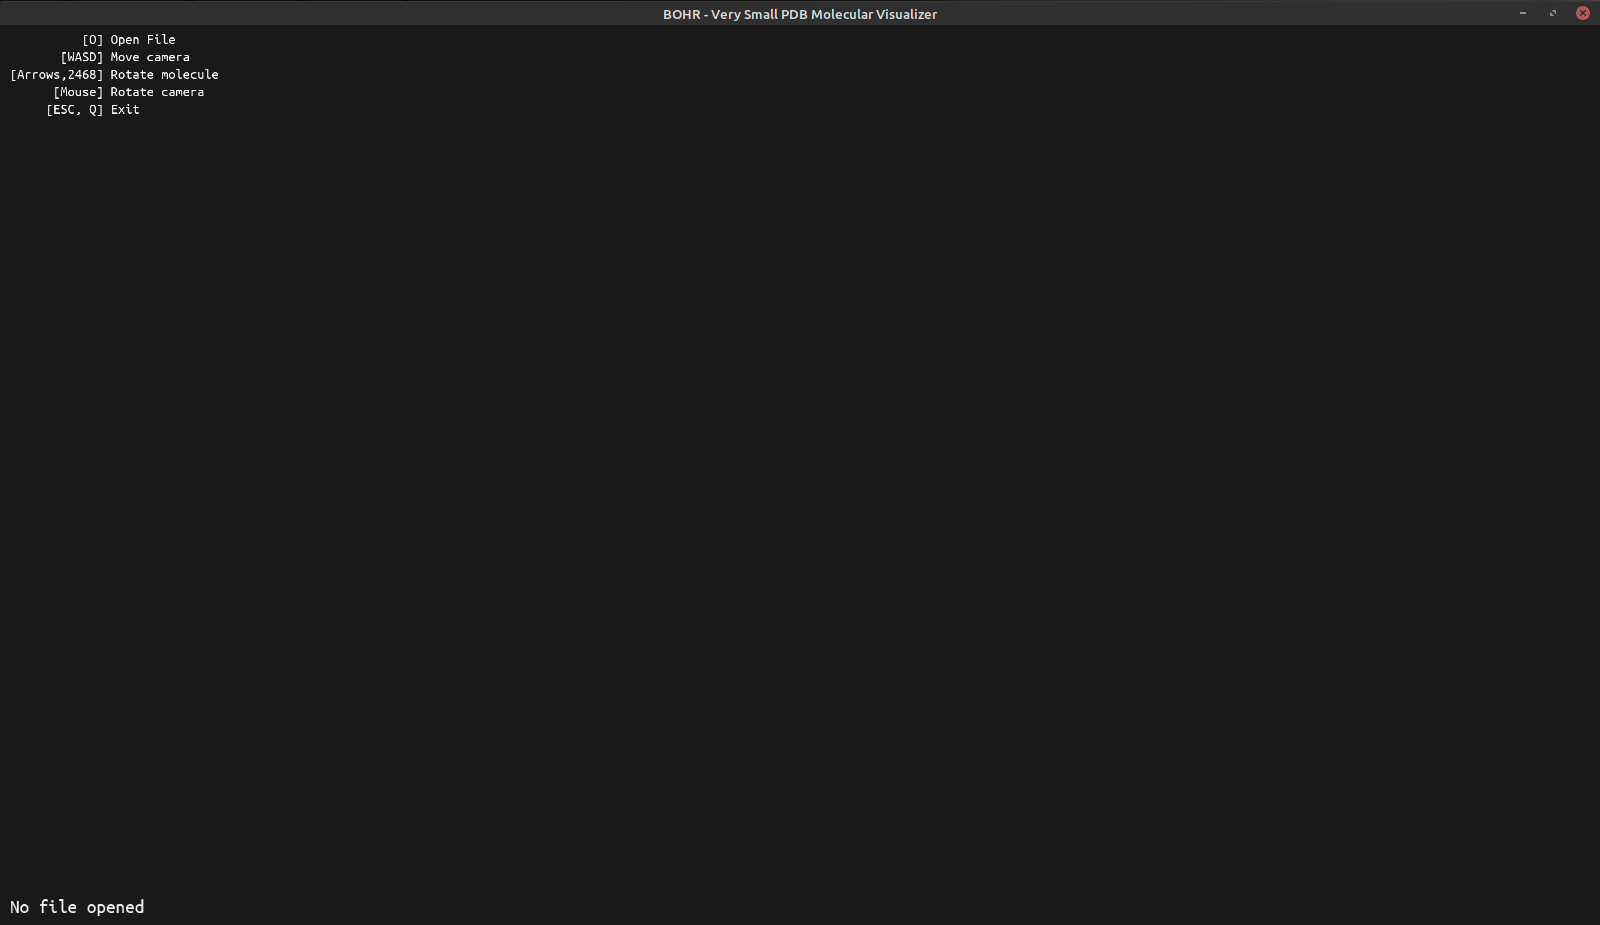
\includegraphics[width=\textwidth]{bohr-start}
    \caption[Aplicação após abertura]{Aplicação após abertura ou quando não tem uma molécula aberta para renderização.}
    \label{fig::bohr-start}
\end{figure}


\begin{figure}[!btp]
    \centering
    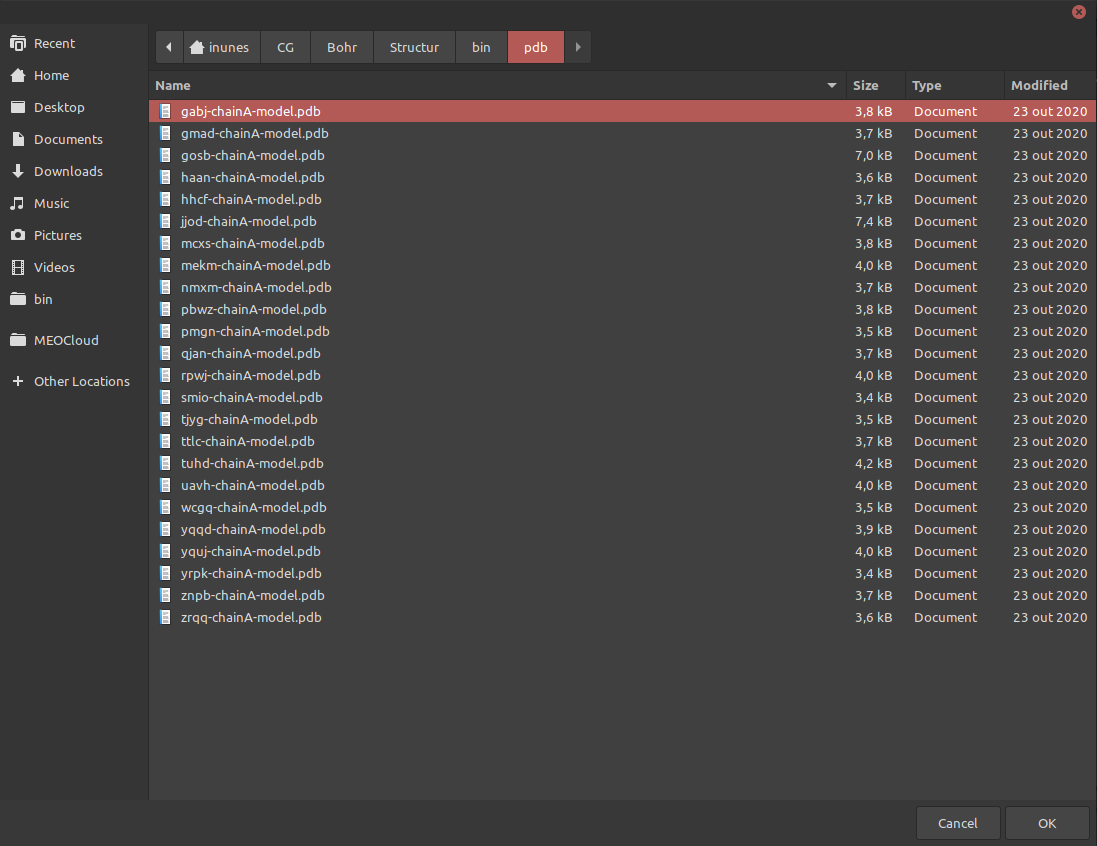
\includegraphics[width=\textwidth]{bohr-opendialog}
    \caption[Janela de diálogo para abertura de ficheiro]{Janela de diálogo do sistema operativo para abertura de um novo ficheiro \ac{PDB}.}
    \label{fig::bohr-opendialog}
\end{figure}


\begin{figure}[!btp]
    \centering
    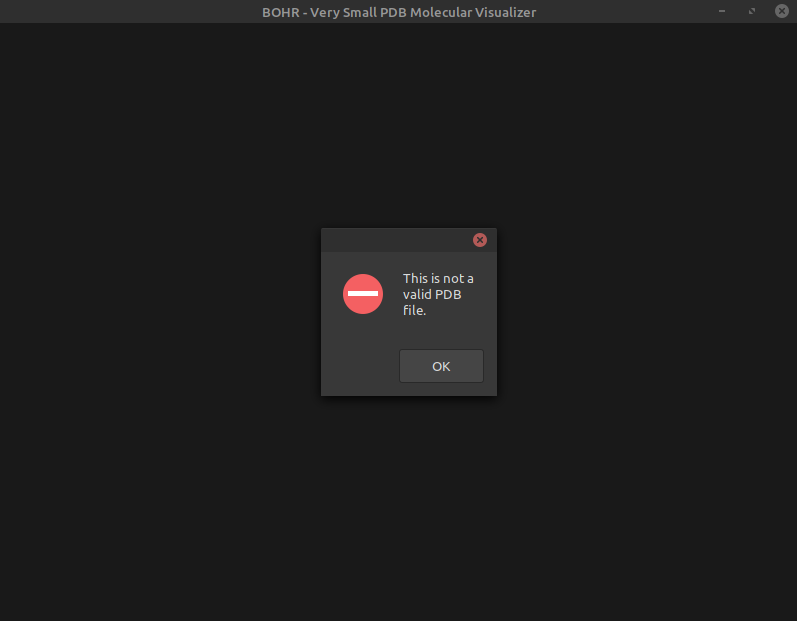
\includegraphics[scale=1.0]{bohr-error}
    \caption[Mensagem de erro]{Mensagem de erro caso o ficheiro não seja válido.}
    \label{fig::bohr-error}
\end{figure}


\begin{figure}[!btp]
    \centering
    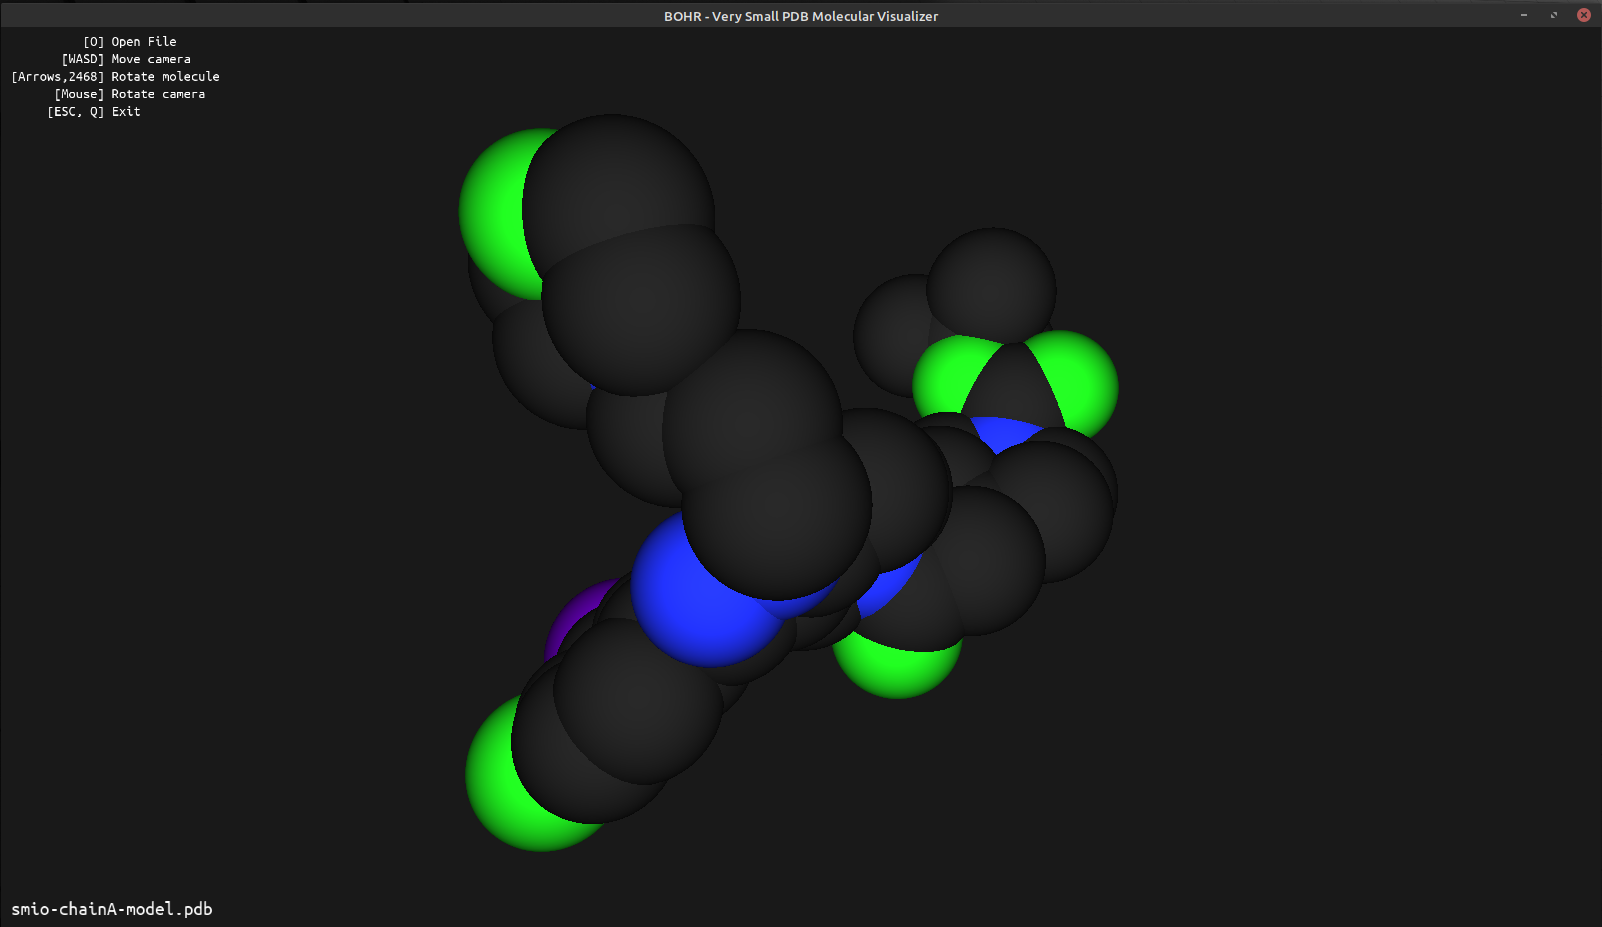
\includegraphics[width=\textwidth]{bohr-main}
    \caption[Exemplo de molécula renderizada]{Exemplo de uma molécula renderizada na aplicação após interpretação do ficheiro \ac{PDB}.}
    \label{fig::bohr-main}
\end{figure}

%\clearpage{\thispagestyle{empty}\cleardoublepage}
\chapter{Reflexão Crítica e Problemas Encontrados}
\label{ch::reflexao}

\section{Introdução}
\label{sec::reflexao:intro}

Não obstante o planeamento feito \textit{a priori}, o projeto \theapp, tal como qualquer outro na área das \ac{TI}, enfrentou alguns contratempos e, devido a problemas de saúde e pessoais severos por parte de um dos membros do grupo, não se revelou possível almejar todas as ambições inicialmente imaginadas. É preciso, pois, refletir sobre o desenvolvimento deste projeto.

Neste Capítulo são, portanto, explorados os seguintes tópicos:

\begin{itemize}
	\item Objetivos propostos vs. alcançados (Secção \ref{sec::reflexao:objetivos}): compara os objetivos inicialmente propostos com aqueles que foram concluídos no projeto final;
	\item Divisão de trabalho pelos elementos do grupo (Secção \ref{sec::reflexao:divisao}): lista as tarefas realizadas por cada elemento da equipa;
	\item Problemas encontrados (Secção \ref{sec::reflexao:problemas}): na sequência da Secção \ref{sec::reflexao:objetivos}, explora os problemas encontrados durante a implementação da aplicação;
	\item Reflexão crítica (Secção \ref{sec::reflexao:critica}): é feita uma \ac{SWOT} em retrospetiva pela equipa acerca do projeto.
\end{itemize}



\section{Objetivos Propostos vs. Alcançados}
\label{sec::reflexao:objetivos}

A Tabela \ref{tab::objetivos} expõe os objetivos propostos inicialmente para o projeto e identifica quais foram alcançados na sua plenitude, quais foram alcançados apenas parcialmente, e quais não tiveram sucesso.

\begin{table}[!htbp]
	\centering
	\begin{tabular}{p{.65\textwidth} >{\centering\let\newline\\\arraybackslash\hspace{0pt}}m{.25\textwidth}}
		\toprule
		{\bfseries Objetivo proposto} & {\bfseries Alcançado?} \\
		\midrule
		\textit{Parsing} de ficheiros \acs{PDB}              & $\bullet$ \\
		Computação das esferas                               & $\bullet$ \\
		Obtenção do raio de cada átomo                       & $\bullet$ \\
		Obtenção da cor CPK de cada átomo                    & $\bullet$ \\
		Renderização de uma esfera                           & $\bullet$ \\
		Renderização de uma molécula                         & $\bullet$ \\
		Rotação de uma molécula                              & $\bullet$ \\
		Movimentação da câmara                               & $\bullet$ \\
		Abertura dinâmica de ficheiros por interface gráfica & $\bullet$ \\
		Renderização da superfície de \textit{van der Walls} & $\bullet$ \\
        Suporte a proteínas                                  & $\circ$   \\
        Renderização da superfície implícita \textit{pi}     & --        \\
        Utilização regular do \textit{Trello}                & --        \\
		\bottomrule
	\end{tabular}
	\caption[Objetivos propostos vs. alcançados]{
		Objetivos propostos e respetiva indicação de sucesso.\\
		\textit{Legenda.} $\bullet$ Alcançado em pleno; $\circ$ Alcançado parcialmente. -- Não alcançado.
	}
	\label{tab::objetivos}
\end{table}


\begin{table}[!htbp]
	\centering
	\begin{tabular}{l c c}
		\toprule
		\textbf{Tarefa} & \textbf{DS} & \textbf{IN} \\
		\midrule
        \textit{Parsing} de ficheiros \acs{PDB}              &  & $\bullet$ \\
        Computação das esferas                               &  & $\bullet$ \\
        Obtenção do raio de cada átomo                       & $\bullet$ &  \\
        Obtenção da cor CPK de cada átomo                    & $\bullet$ &  \\
        Renderização de uma esfera                           &  & $\bullet$ \\
        Renderização de uma molécula                         &  & $\bullet$ \\
        Rotação de uma molécula                              & $\bullet$ &  \\
        Movimentação da câmara                               & $\bullet$ &  \\
        Abertura dinâmica de ficheiros por interface gráfica &  & $\bullet$ \\
        Renderização da superfície de \textit{van der Walls} &  & $\bullet$ \\
		\bottomrule
	\end{tabular}
	\caption[Distribuição de tarefas]{
		Distribuição de tarefas pelos elementos do grupo.\\
		\textit{Legenda.}~%
		$\bullet$ principal responsável; $\circ$ auxiliou.
		DS: Diogo Simões; IN: Igor Nunes.
	}
	\label{tab::divisao-trabalho}
\end{table}


\section{Divisão de Trabalho pelos Elementos do Grupo}
\label{sec::reflexao:divisao}

A fim de agilizar o desenvolvimento do projeto, as tarefas foram distribuídas de forma balanceada pelos dois elementos da equipa (Tabela \ref{tab::divisao-trabalho}). De notar que, apesar da divisão de tarefas, a participação do grupo no seu todo foi essencial nos momentos de entreajuda, esclarecimento de dúvidas e consolidação da aplicação final.

% Reuniões semanais foram realizadas com \textit{deadlines} bem definidas para cada tarefa, tendo sido realizadas reuniões extraordinárias em momentos críticos do desenvolvimento.



\section{Problemas Encontrados}
\label{sec::reflexao:problemas}

A implementação da aplicação levou a que o grupo encontrasse alguns problemas e contratempos, os quais teve de ultrapassar a fim de terminar o projeto. Os problemas mais notáveis são resumidos na Tabela \ref{tab::problemas}, incluindo as soluções encontradas para os ultrapassar.

\begin{table}[!htbp]
	\centering
	\begin{tabular}{p{.36\textwidth} p{.56\textwidth}}
		\toprule
		{\bfseries Problema} & {\bfseries Solução} \\
		\midrule
		\midrule
        \textit{Parsing} dos ficheiros \ac{PDB}. & Estudo do formato segundo descrito em diversos fóruns \textit{online} a fim de determinar as posições exatas dos dados relativo a cada átomo. \\
        \midrule
		Procura do método mais eficiente para renderizar uma esfera. & Utilização da classe \textit{Sphere} disponibilizada no \textit{OpenGL Shading Language Cookbook, 2nd Edition} \cite{vbosphere} a fim de evitar a importação de objetos externos. \\
		\midrule
		Determinação da superfície implícita \textit{pi}. & Sem solução encontrada. É necessário mais estudo. \\
		\midrule
		Renderização da superfície implícita \textit{pi} e dificuldade do algoritmo \textit{marching cubes}. & Adoção do algoritmo \textit{marching triangles} com recurso ao código \textit{open source} disponível em \cite{marchingtriangles}. Solução não presente na aplicação final devido ao problema anterior não solucionado. \\
		\bottomrule
	\end{tabular}
	\caption[Problemas encontrados e respetivas soluções]{Problemas encontrados durante o desenvolvimento da aplicação e respetivas soluções adotadas.}
	\label{tab::problemas}
\end{table}



\section{Reflexão Crítica}
\label{sec::reflexao:critica}

Tendo por objetivo expor a reflexão da \groupname~face ao trabalho enveredado no desenvolvimento da aplicação \theapp, propõe-se efetivá-la com uma análise \ac{SWOT}.

\subsection{Pontos Fortes}
\label{ssec::reflexao:critica:fortes}

\begin{enumerate}[nosep]
	\item A aplicação permite abrir uma nova molécula a qualquer momento.
    \item É utilizada interface gráfica do sistema operativo para interagir com o utilizador.
    \item As esferas são calculadas dinamicamente pela aplicação sem recurso a objetos externos.
    \item O renderizador tem em conta a cor de cada átomo e o respetivo raio de \textit{van der Walls}, mostrando assim a superfície de \textit{van der Walls}.
\end{enumerate}


\subsection{Pontos Fracos}
\label{ssec::reflexao:critica:fracos}

\begin{enumerate}[nosep]
	\item O \textit{parser} \ac{PDB} não contempla ficheiros relativos a proteínas.
    \item O mesmo código-fonte compilado em diferentes sistemas operativos não garante exatamente o mesmo comportamento em relação à câmara e ao teclado.
    \item Não é calculada a superfície implícita \textit{pi}, não sendo então possível renderizar esta.
    \item Só é renderizado um tipo de superfície molecular.
\end{enumerate}


\subsection{Ameaças}
\label{ssec::reflexao:critica:ameacas}

\begin{enumerate}[nosep]
	\item O \textit{software} não contempla a possibilidade de fechar a molécula atualmente aberta nem se mostrar várias moléculas lado-a-lado.
    \item O uso de interface gráfica não tem um comportamento garantido em \textit{cross-platform}.
    \item Para moléculas de grandes dimensões, a aplicação poderá facilmente tornar-se exigente em termos de recursos de memória.
    \item Já existem variados \textit{softwares} de visualização molecular, apesar da pertinência deste projeto no âmbito da \ac{UC} de \ac{CG}.
\end{enumerate}


\subsection{Oportunidades}
\label{ssec::reflexao:critica:oportunidades}

\begin{enumerate}[nosep]
	\item Adicionar suporte para aminoácidos.
    \item Adaptar com \textit{flags} do pré-processador do C++ o código-fonte a fim de ultrapassar as limitações em cada sistema operativo.
    \item Determinar a superfície implícita \textit{pi} a fim de dar uso ao algoritmo \textit{marching triangles} estudado para este projeto.
    \item Renderizar mais superfícies, tendo em conta os vários raios armazenados na tabela periódica interna da aplicação.
\end{enumerate}



\section{Notas finais}
\label{sec::reflexao:notas}

Antes de terminar a reflexão crítica, é pertinente levar em conta os problemas pessoais e de saúde enfrentados por cada um dos membros do grupo que acabou por levar a um significativo atraso da conclusão do projeto face à data prevista.

O grupo reconhece, portanto, este mesmo atraso, o qual culminou no não cumprimento total dos objetivos inicialmente propostos para este projeto.

Não obstante, o facto de esta aplicação ter por base op cálculo e a renderização dinâmica de todos os seus elementos, ao invés de uma abordagem \textit{hard-coded}, levantou novos desafios até então não encontrados durante as aulas práticas da \ac{UC} de \ac{CG}.

Consideramos, portanto, que, apesar do lamentável atraso, o resultado final obtido é satisfatório.


\section{Conclusões}
\label{sec::reflexao:conclusao}

Esta fase de reflexão permitiu analisar o trabalho enveredado ao longo das semanas de planeamento, execução e teste. Com esta análise, a equipa pôde tirar conclusões não só sobre o seu desempenho, mas também acerca das tecnologias utilizadas, as quais serão expostas no Capítulo seguinte.

%\clearpage{\thispagestyle{empty}\cleardoublepage}
\chapter{Conclusões e Trabalho Futuro}
\label{ch::conclusao}

\section{Conclusões Principais}
\label{sec::conclusao:principal}

Text\ldots


\section{Trabalho Futuro}
\label{sec::conclusao:futuro}

Text\ldots

%\clearpage{\thispagestyle{empty}\cleardoublepage}

% SE EXISTIREM APENDICES, DESCOMENTAR O QUE ESTÁ EM BAIXO
%\pagenumbering{Alph}

\appendix
% \include{chatbot}
% \clearpage{\pagestyle{empty}\cleardoublepage}
% \include{codigo}
% \clearpage{\pagestyle{empty}\cleardoublepage}
% \include{apendice2}
% \clearpage{\pagestyle{empty}\cleardoublepage}
% \include{apendice3}
% \clearpage{\pagestyle{empty}\cleardoublepage}

\backmatter

% \bibliographystyle{plain}
\bibliographystyle{IEEEtran}
\bibliography{bibliografia}

\end{document}